

\section{Introdução aos SMAs}

\begin{frame}

  \frametitle{Motivando aos SMAs}
    
    
\begin{figure}[!ht]
\centering
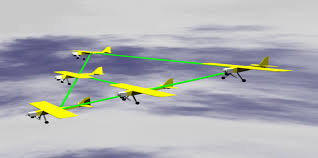
\includegraphics[height =.6\textheight,width=.7\textwidth]{figuras/agentes_vizinhos01.jpeg}
\caption{Observe o sentido das flechas --  e  o foco da missão}
%\label{ag_01}
\end{figure}
    
    
\end{frame}


\begin{frame}
\frametitle{Motivando aos SMAs}

\begin{figure}[!ht]
\centering
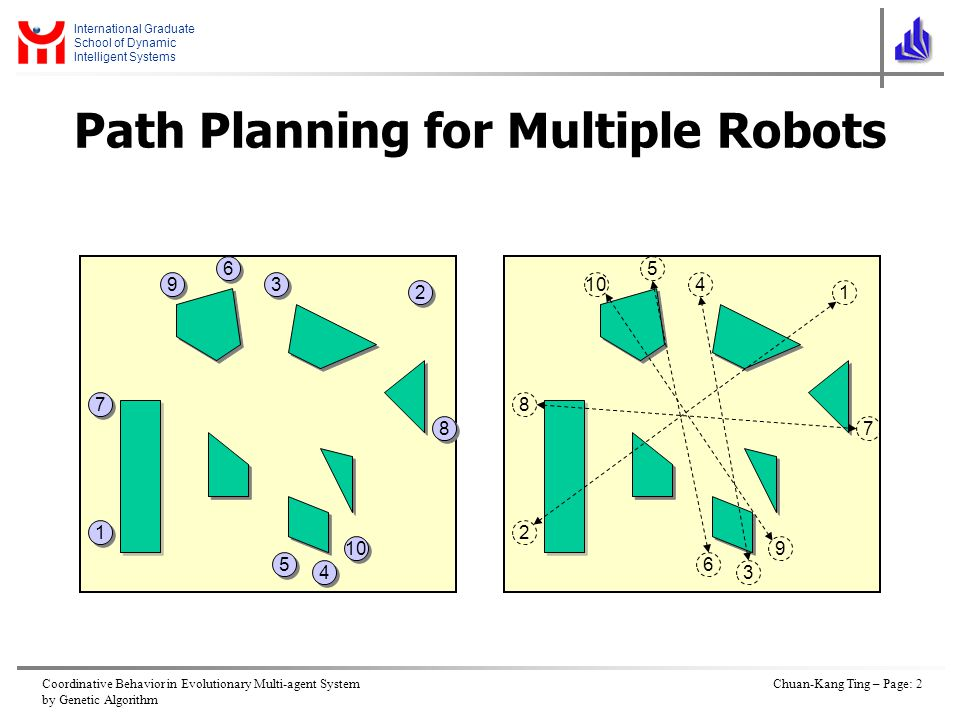
\includegraphics[height =.6\textheight,width=.7\textwidth]{figuras/agentes_vizinhos02.jpeg}
%\caption{Arquitetura clássica}
%\label{ag_01}
\end{figure}
\end{frame}
%%%%%%%%%%%%%%%%%%%%%%%%%%%%%%%%%%%%%%%%%%%%%%%%%%%%%%%%%%%%%%%%%

\begin{frame}

  \frametitle{Motivando aos SMAs}

\begin{figure}[!ht]
\centering
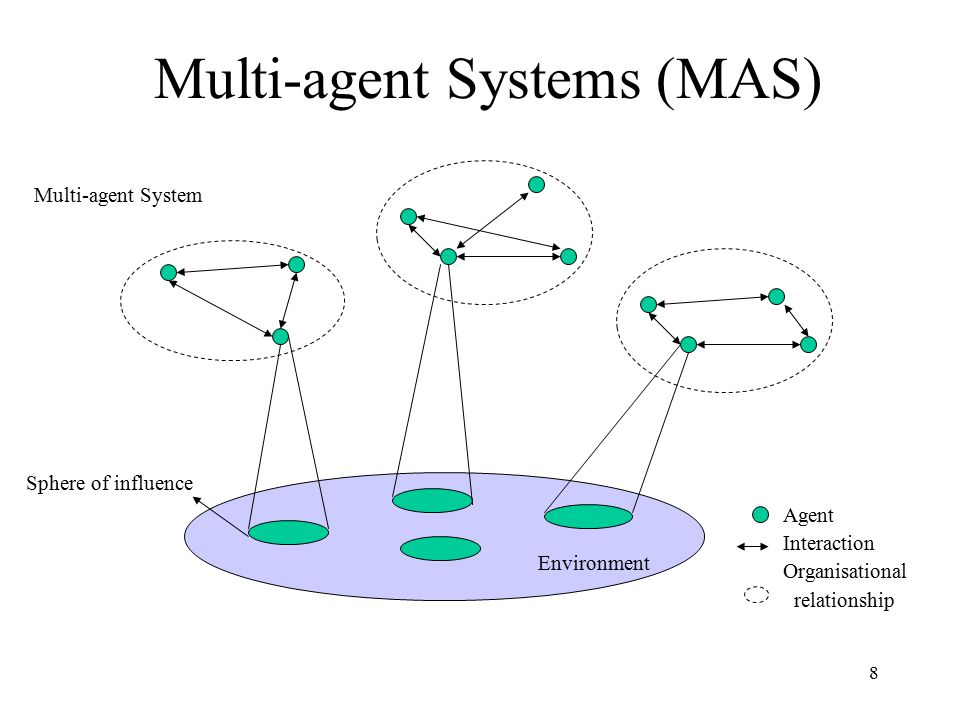
\includegraphics[height =.6\textheight,width=.7\textwidth]{figuras/agentes_vizinhos03.jpeg}
\caption{Arquitetura clássica -- comunidade de agentes $\equiv $   SMA}
%\label{ag_01}
\end{figure}
 
\end{frame}
%%%%%%%%%%%%%%%%%%%%%%%%%%%%%%%%%%%%%%%%%%%%%%%%%%%%%%%%%%%%%%%%%


\subsection{Motivação aos SMAs}
\begin{frame} [allowframebreaks=0.9]

    \frametitle{Motivação I}
    Projetar e construir sistemas multiagentes é uma tarefa difícil, pois:
    \begin{itemize}
    \pause
      \item Apresenta todos os problemas já conhecidos 
dos sistemas distribuídos e concorrentes.
\pause
      \item Dificuldades adicionais surgem da flexibilidade 
e complexidade das interações
    
    \end{itemize}
\end{frame}



\begin{frame}
\frametitle{Esta complexidade por um DFD por agente x ações:}
  
  \begin{figure}[!ht]
  \centering
  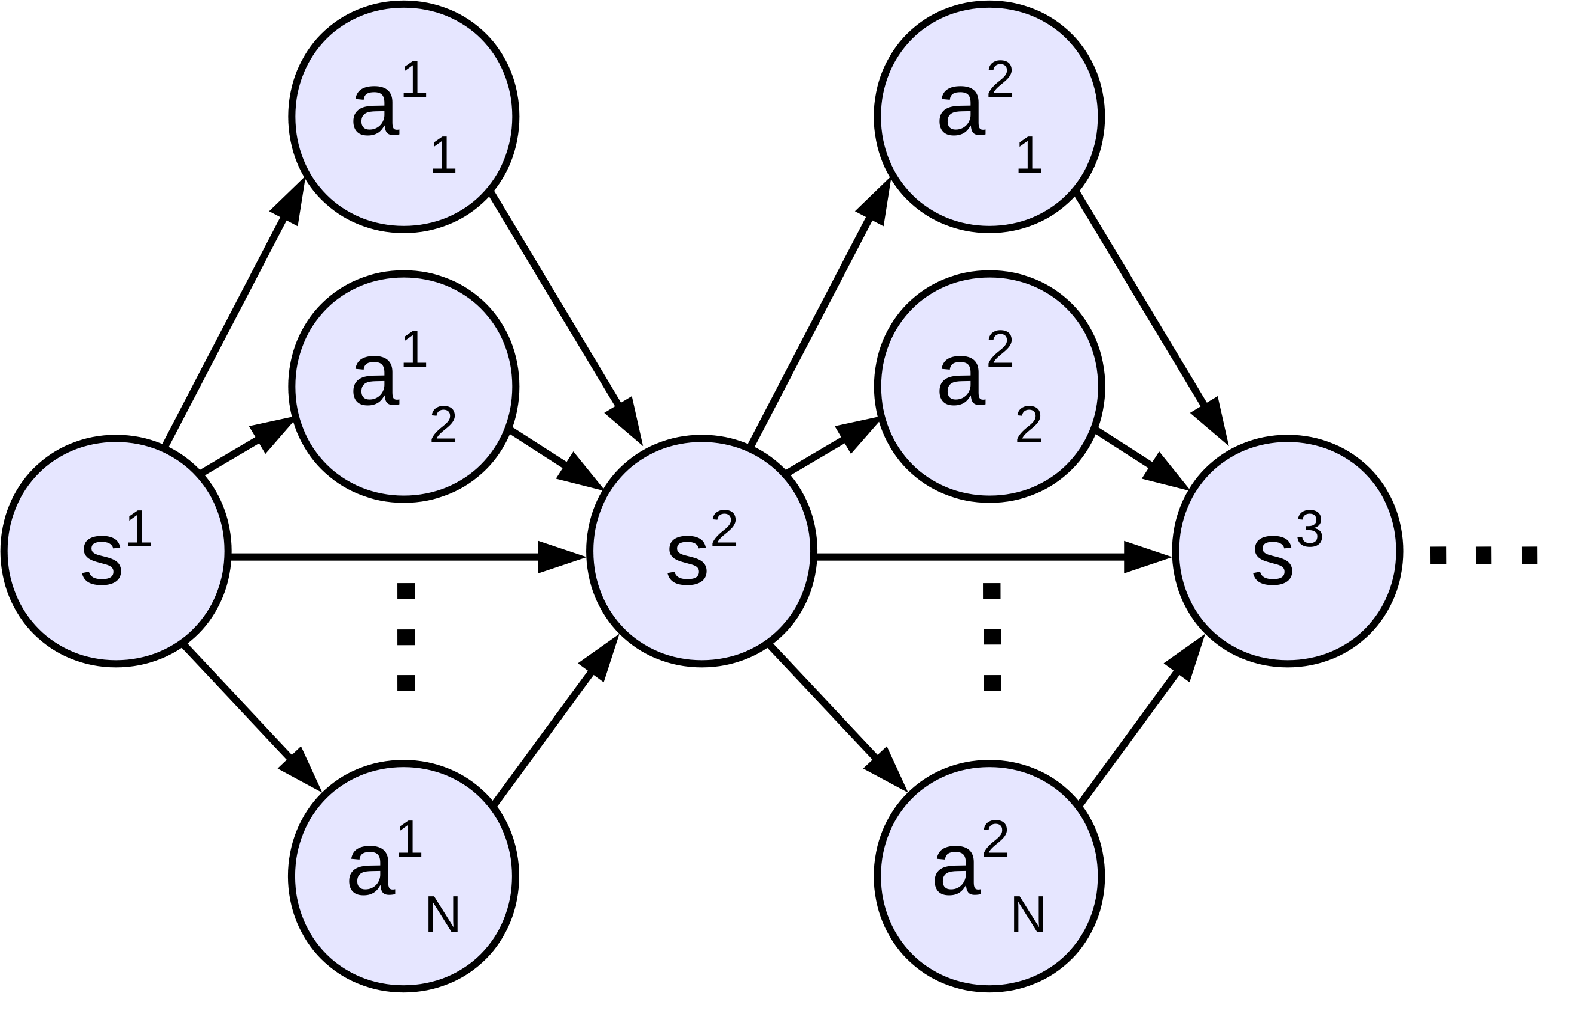
\includegraphics[height =.6\textheight,width=.7\textwidth]{figuras/mudando_estados01.png}
  \caption{Complexidade via DFD de um SMA (agentes) $\times $ ações $\equiv $ um único estado}
%\label{ag_01}
\end{figure}
   
\end{frame}




\begin{frame}

    \frametitle{Motivação II}
   Dois principais impedimentos técnicos, pois:
    \begin{itemize}
    \pause
      \item Inexistência de uma metodologia sistemática para 
      claramente especificar e estruturar aplicações SMA.
     \pause
      \item Inexistência de ferramentas e ambientes de 
desenvolvimento de SMA com qualidade industrial.
    
    \end{itemize}
\end{frame}

%%%%%%%%%%%%%%%%%%%%%%%%%%%%%%%%%%%%%%%%%%%%%%%%%%%%%%%%%%%%%%%%%%%%%%%%

\subsection{Os Elementos de SMAs}



\begin{frame}[allowframebreaks=0.9]

    \frametitle{Os Elementos de SMAs}
   
   \begin{description}
     \item[Projeto de Agente:] 
     
    \item[Ambiente:]
          
   \item[Percepção:]
               
 \item[Controle:]
                    
  \item[Conhecimento:]
                          
  \item[Comunicação:]
          
   \end{description}
   
   
\end{frame}


